\documentclass{article}

\usepackage[final]{nips_2016}

\usepackage[utf8]{inputenc} % allow utf-8 input
\usepackage[T1]{fontenc}    % use 8-bit T1 fonts
\usepackage{hyperref}       % hyperlinks
\usepackage{url}            % simple URL typesetting
\usepackage{booktabs}       % professional-quality tables
\usepackage{amsfonts}       % blackboard math symbols
\usepackage{nicefrac}       % compact symbols for 1/2, etc.
\usepackage{microtype}      % microtypography
\usepackage{graphicx}       % figures
\usepackage{epstopdf}       % for pdf

\title{Synaptic Density Distribution in the Cortex}

\author{
  Bijan K. Varjavand\\
  Johns Hopkins University\\
  3510 N Charles St. Baltimore, MD 21218 \\
  \texttt{bvarjav1@jhu.edu} \\
}

\begin{document}

\maketitle

\begin{abstract}
  The brain is an incredibly complicated organ in the human body, 
  and we do not understand almost anything about how it functions. 
  We can, however, analyze its physical characteristics. Here, we 
  can see huge numbers of neurons and synapses bundled together. 
  The state of these neurons and synapses are hugely important to 
  diagnosing illnesses and diseases. This paper seeks to go more 
  in depth into the synaptic density distribution in the brain.
\end{abstract}

\section{Introduction}

Many papers have already been published based on the specific characteristics of these neurons and synapses, looking at their behavior in different environments. For example, it has been found that sufferers of Alzheimer's have a lower synaptic density than usual, and many have found correlations between the two (Scheff 1990; Koffie et al. 2011). Further analysis may provide additional insight to solutions for these problems.

\subsection{The opportunity at hand}

Even with previous technology from before the 21st century, the field of using EM to analyze synapses was bustling (Van Horn, et al. 2000). With the advent of more and more sophisticated imaging techniques and viewing tools, the number of conclusions that we can draw from EM images grows increasingly larger (paper). Other techniques for imaging are rapidly being developed that provide a higher resolution imaging (Dani, et al. 2010; Merchant, et al. 2015). This makes way for an unprecedented opportunity to learn more about the brain than what one previously thought possible. The only obstacles left to cross in order to uncover these new features are handling this new huge size of data as well as utilizing an appropriate analytic tool for it.

These obstacles are not easy to overcome - the large data sets that are now available span and exceed TB. Techniques of downsampling are helpful, but only with a thorough investigation of the data can it be done confidently. The analytic tools and algorithms already exist, but their specific applications to each data set vary. One must have some expertise in order to apply relevant algorithms.

\subsection{Filling the gap}

I took the approach of a data scientist, utilizing previous data refinement, asking specific exploratory questions and searching for feature trends in the data. The question on significance of synapses in the brain have myriad answers, I simply strove to apply my own knowledge to these new data sets in search of a refined model of the brain. The numerous data sets to come all still require analysis, and even this data set cannot be said to be thoroughly analyzed. In the future, the number of opportunities will only increase.

\section{Results}

The analytic investigation in the data revealed some interesting features and  trends. First, a manual counting was done to evaluate the synapse counting algorithm. This was assisted by the information in Burette et al.(2015). The first notable conclusion was the slight skew on the data from the algorithm used to count synapses. A manual comparison showed that many synapses failed to be detected across the entire range of the data set. The skew seemed to be affected by changes in x, y, and z values as seen below.

\begin{figure}[h]
  \centering
  \fbox{\rule[-.5cm]{0cm}{4cm} \rule[-.5cm]{4cm}{0cm}}
  \fbox{\rule[-.5cm]{0cm}{4cm} \rule[-.5cm]{4cm}{0cm}}
  \fbox{\rule[-.5cm]{0cm}{4cm} \rule[-.5cm]{4cm}{0cm}}
  \caption{Left: change across x. Center: change across y. Right: change across z.}
\end{figure}

Next, some statistical analysis of the data revealed changes in synapse density across the y axis, while the x and z axes didn't seem to have any visual difference in synapse density across their length.

\begin{figure}[h]
  \centering
  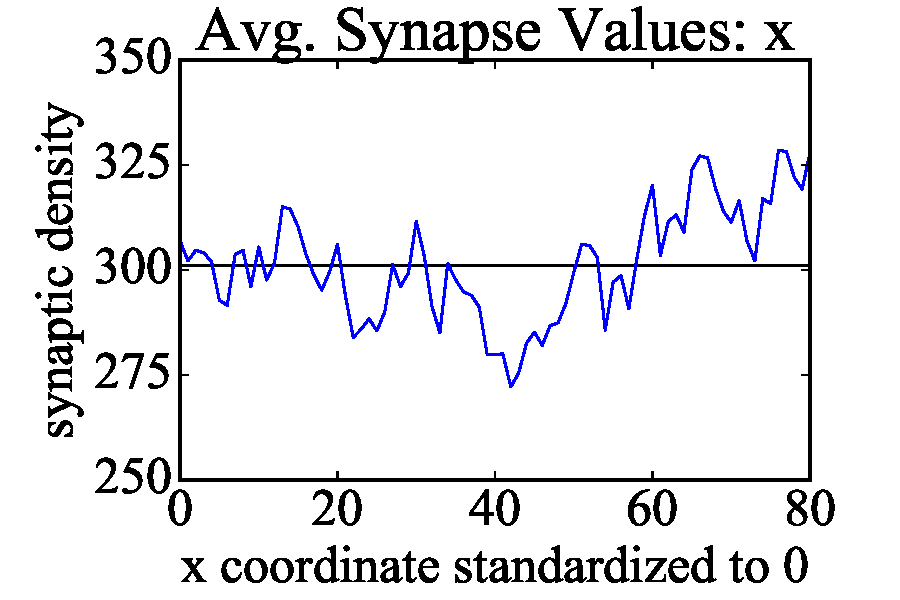
\includegraphics[scale = .3]{Fig2a}
  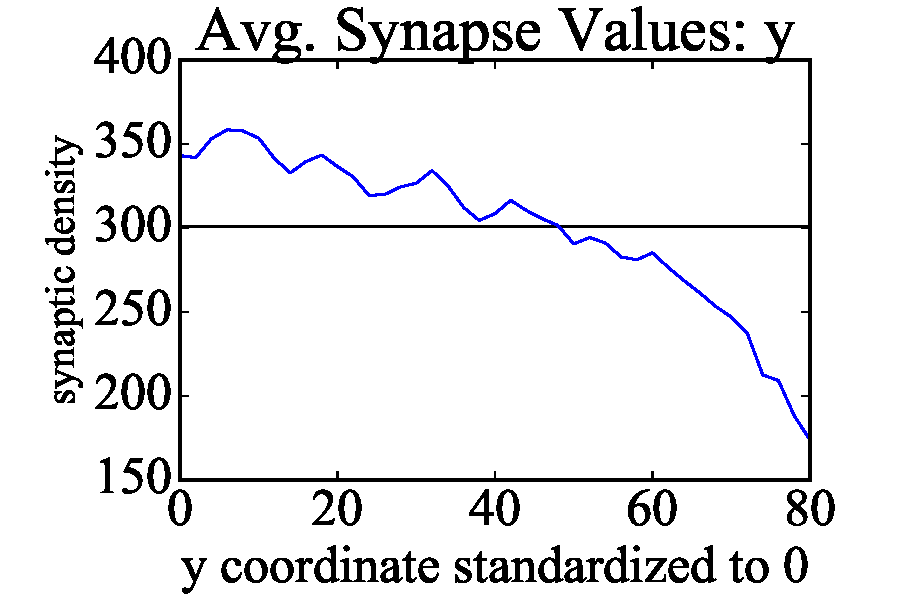
\includegraphics[scale = .3]{Fig2b}
  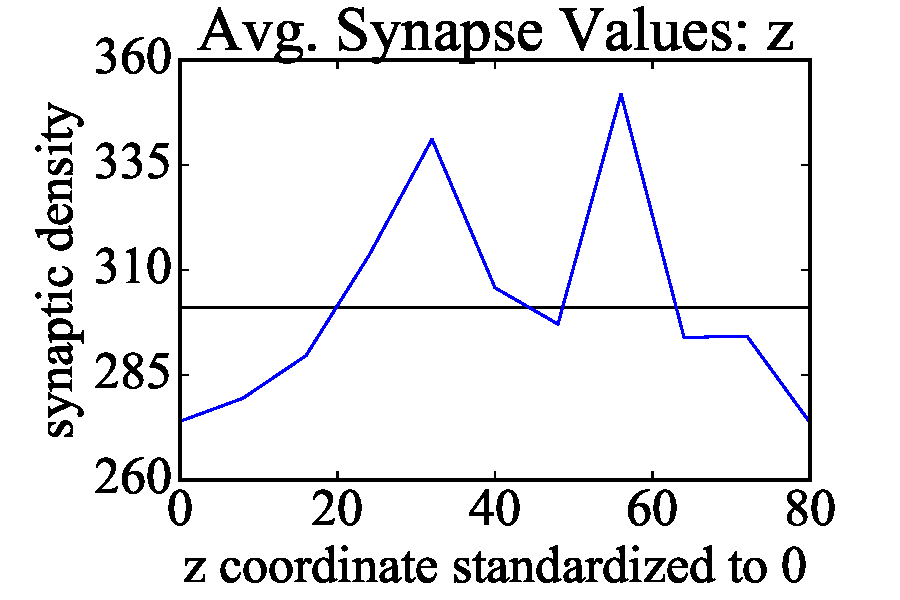
\includegraphics[scale = .3]{Fig2c}
  \caption{Left: synapses across x. Center: synapses across y. Right: synapses across z.}
\end{figure}

Further investigation into synapse density distribution using BIC curves revealed that the data had multiple clusters. Additionally, a spike in the BIC curve across the entire data set at 11 clusters disappeared when BIC curves were generated at each z value. The conclusion that the optimal number of clusters was 4 remained the same across all BIC curves.

\begin{figure}[h]
  \centering
  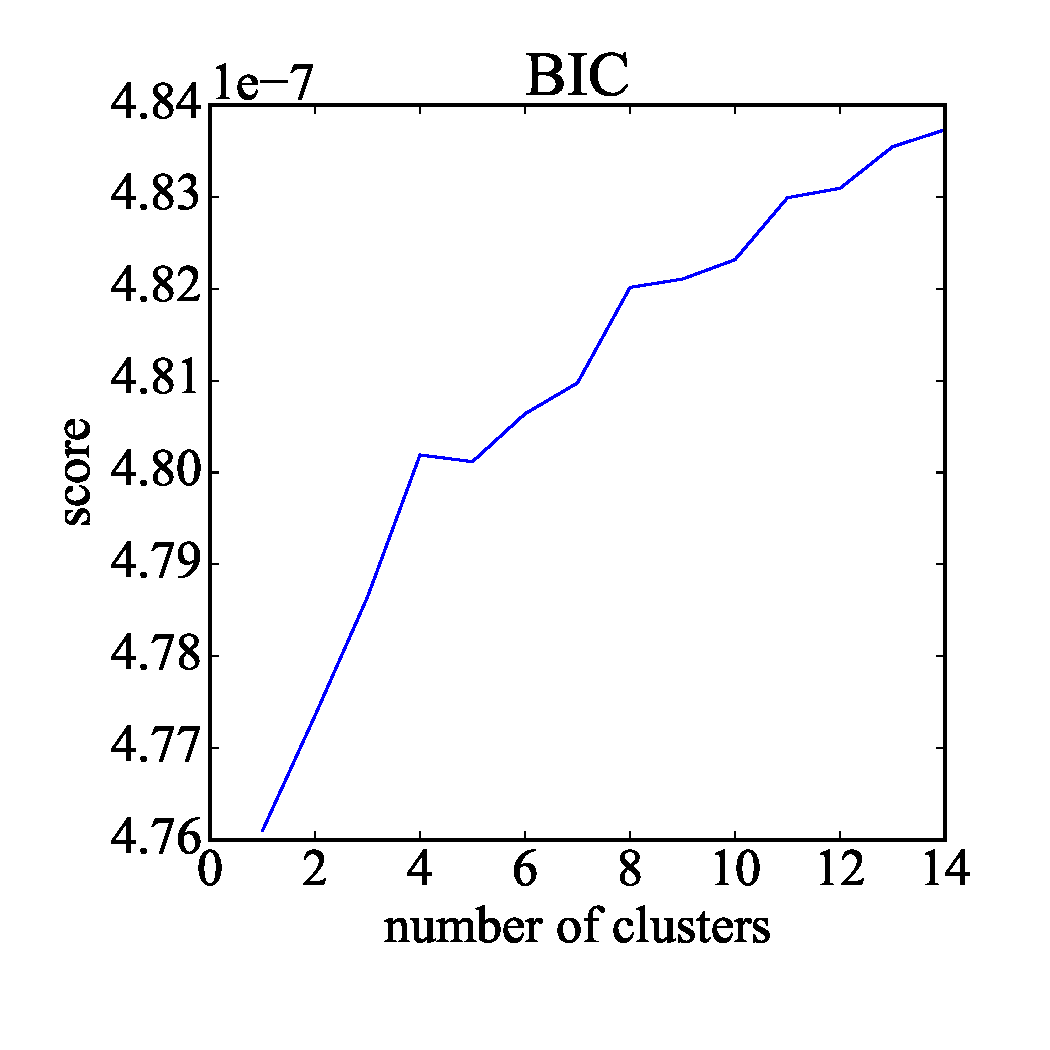
\includegraphics[scale = .3]{Fig10}
  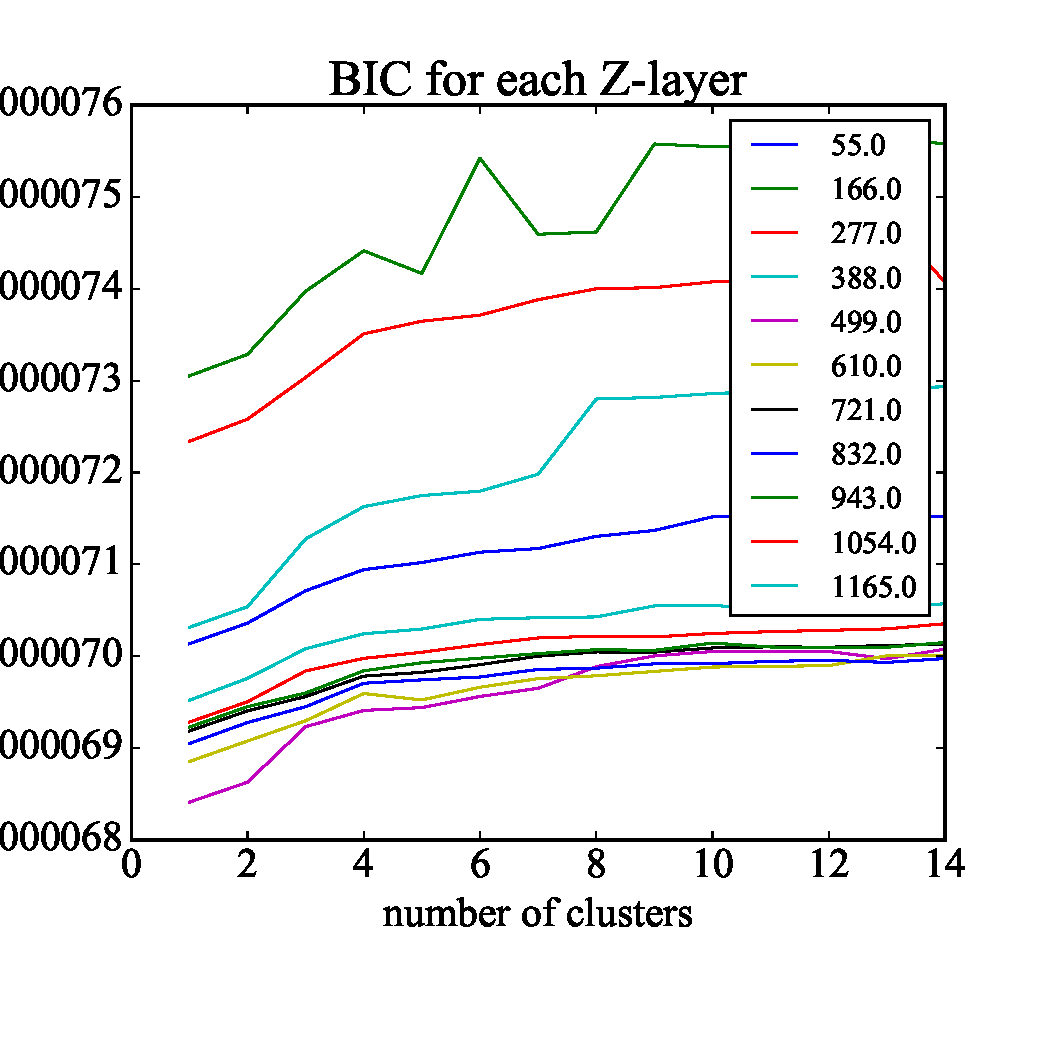
\includegraphics[scale=.3]{Fig12}
  \caption{Left: BIC curve across all data. RightL BIC curve on individual z-values.}
\end{figure}

Finally, k-means clustering confirmed the change in synapse density across z, but also revealed smaller differences in synapse density across other dimensions. In the context of this data set, this could imply that synapse density changes even within cortical layers, not just across them.

\begin{figure}[h]
  \centering
  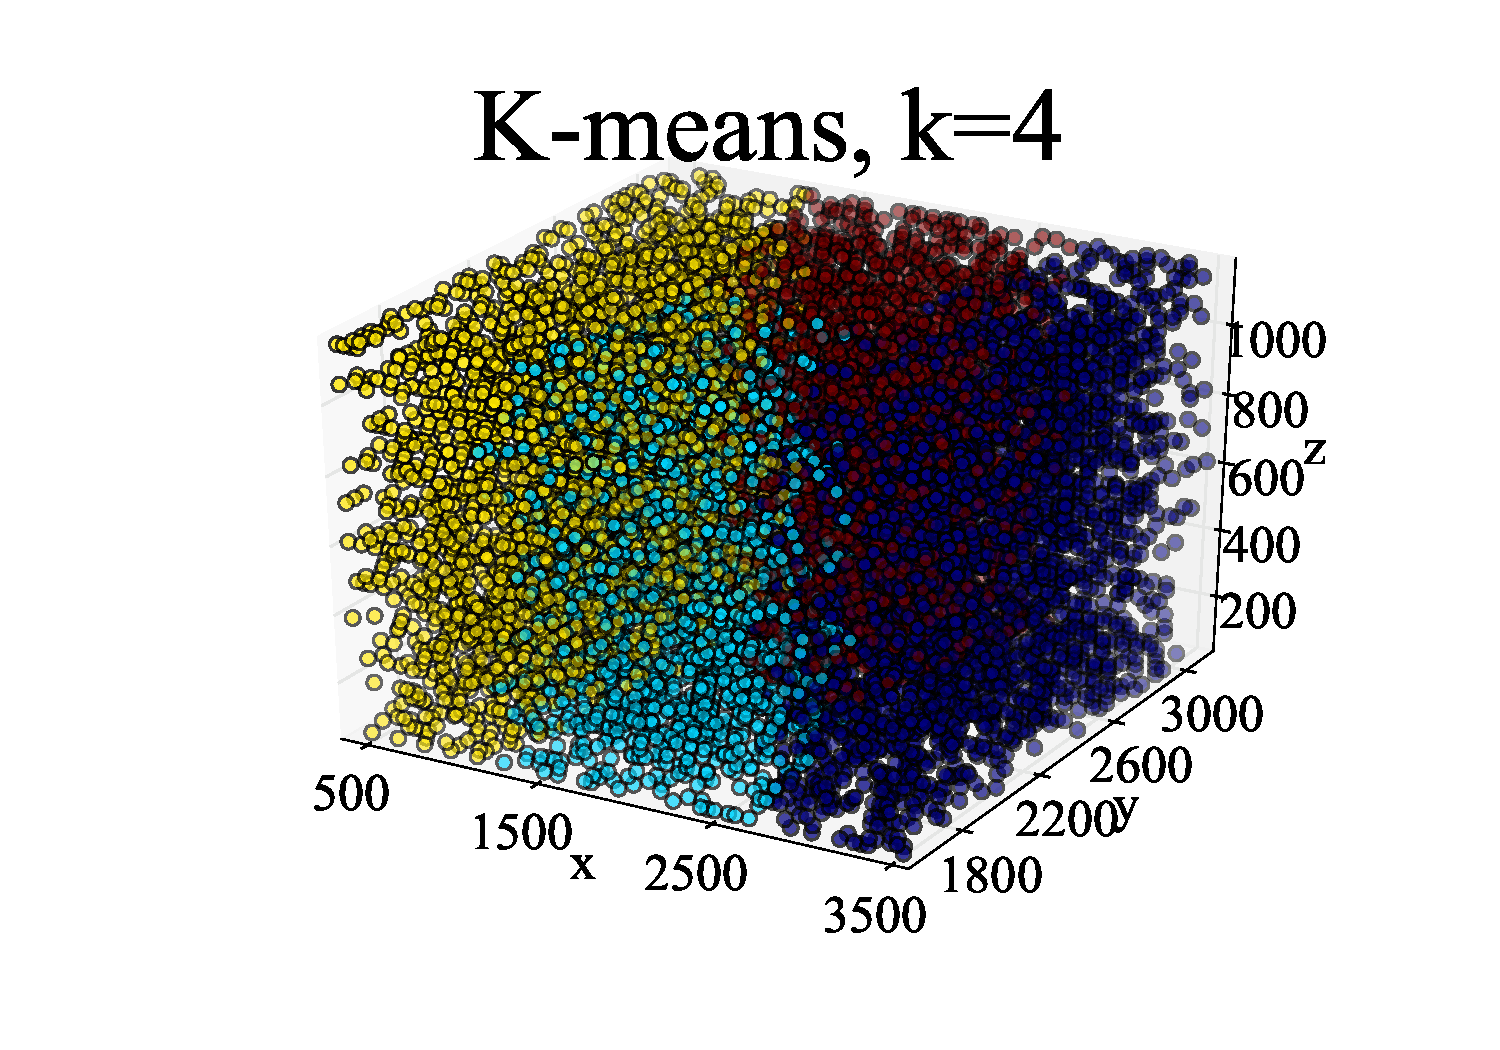
\includegraphics[scale=.15]{Fig13a}
  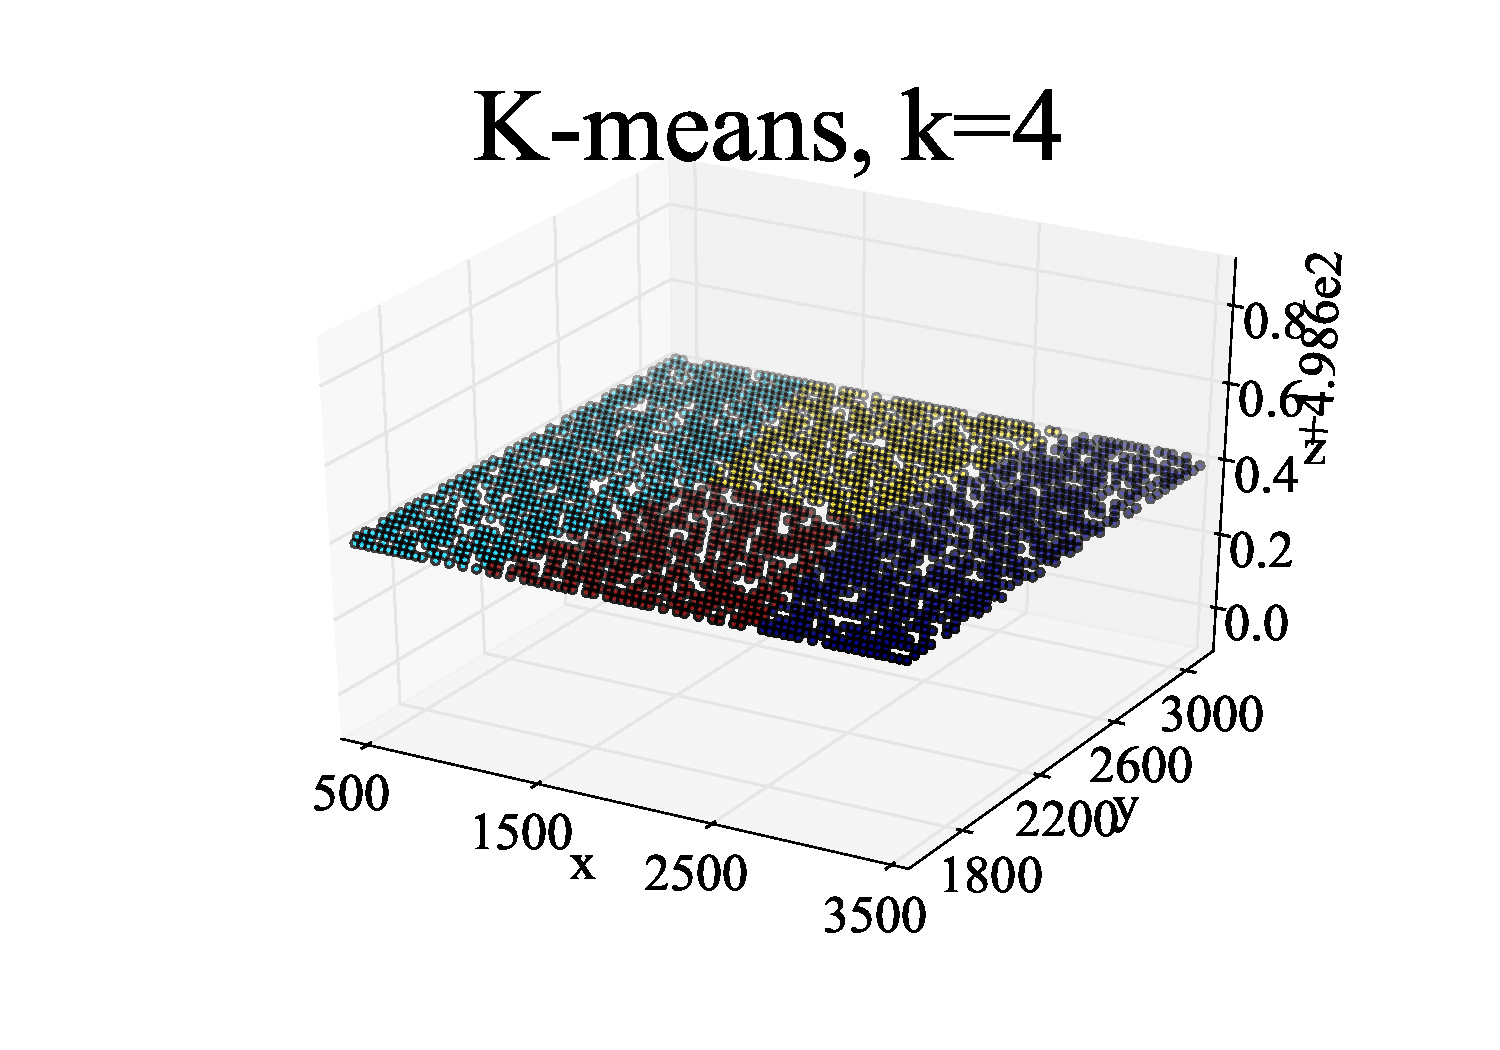
\includegraphics[scale=.15]{Fig13b}
  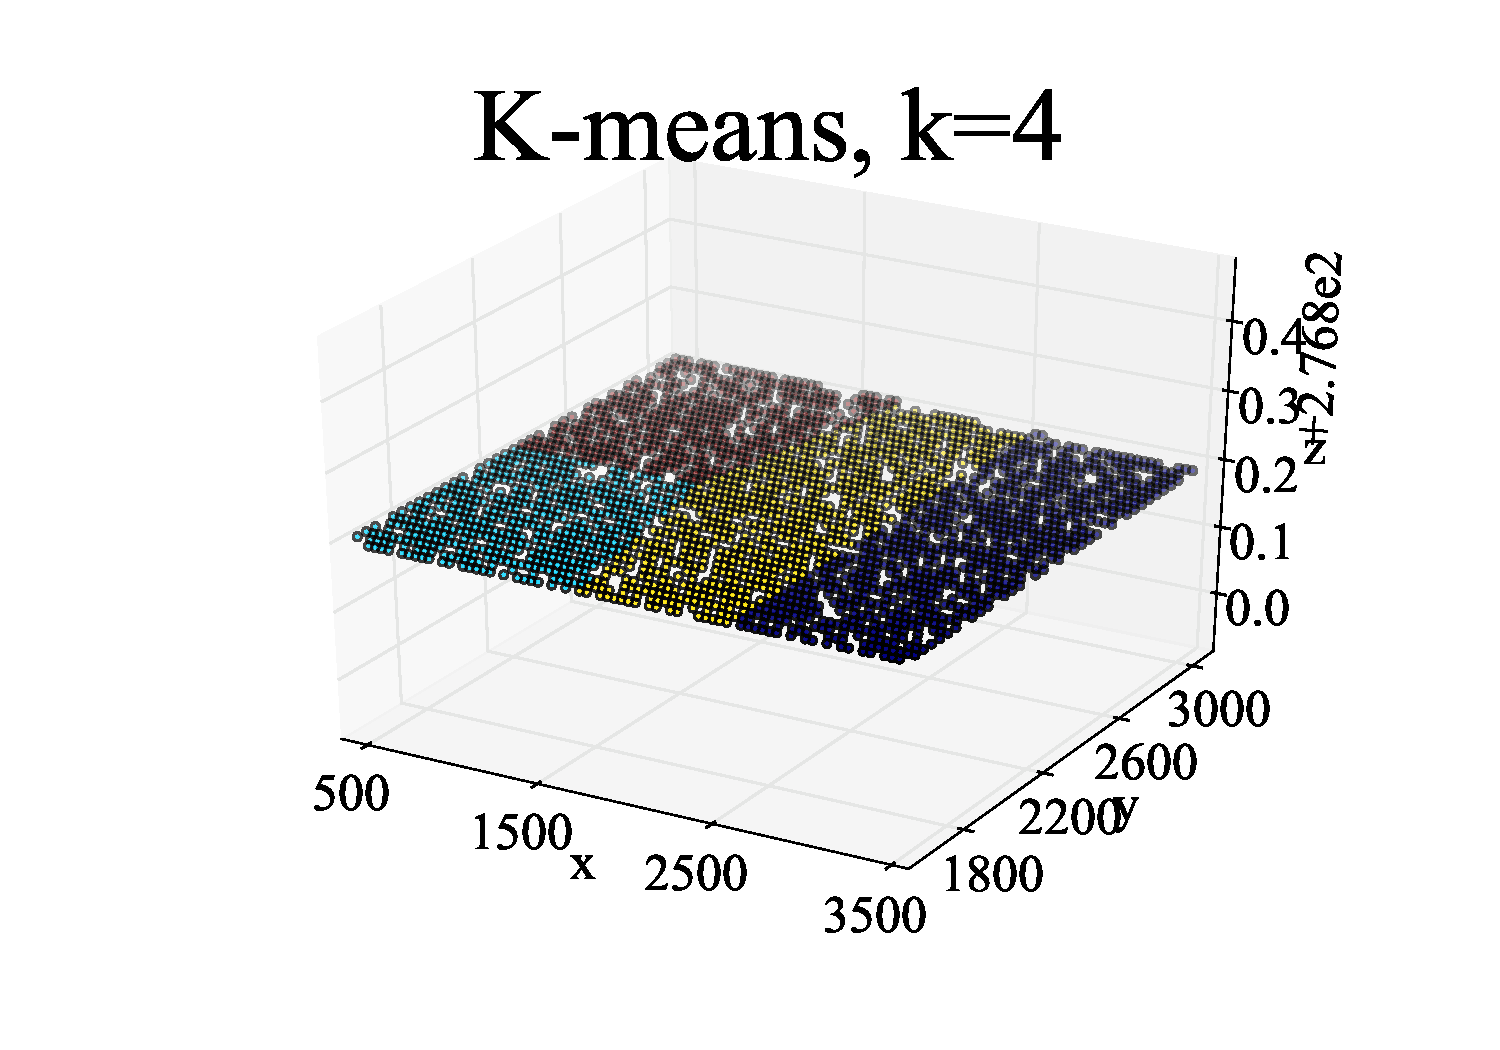
\includegraphics[scale=.15]{Fig13c}
  \caption{K-means in -  Left: entire data set. Center: upper z-values. Right: lower z-values.}
\end{figure}

\section{Methods}

The process of discovering features in a data set required many steps for verification. First, a model was created that represents the data. After initial data screening, initial descriptive analysis was done to generate an overview of the data. Then, assumptions are tested to prepare for an exploratory analysis, which delves deeper into the features to discover.

\subsection{Model}

Each point in our data set is a row vector of length 5, which includes the x, y, and z coordinates as well as an unmasking variable and a synapse variable \[ X_i = [x_i, y_i, z_i, u_i, s_i] \]

\subsection{Data Source}

The data used for this analysis was pulled from
\begin{center}
  \url{http://www.nature.com/nature/journal/v471/n7337/full/nature09802.html}
\end{center}

The data set, after processing and downsampling, created an EM image with voxels 64x64x64 pixels in dimension. A synapse counting algorithm was used to generate a table with 5 columns - 3 for the coordinates, with one for the number of synapses and another for the degree of the voxel's unmasked value. 

After discussions with those familiar to the data set and its method of collection, the definition the "unmasked" value was discovered. This "unmasked" value is simply a term to describe how much of the voxel is unreadable. For example, a value of 0 indicates that none of the voxel is readable, while larger values indicate greater readability of the voxel.

\subsubsection{Cleaning unmasked values of 0}

After an initial overview of the nature of the data, a large number of data points with unmasked values of zero were discovered. These data points are not useful to this approach of analysis as they provide no information. Thus, they were removed from the data set.

\subsubsection{Cleaning edges}

A straightforward look at the data shows that the synapse distribution is significantly different at the edges of the data, where the sample was cut. Therefore, in order to maintain a clean data set free of as much error as possible, data close to the edge of the sample was removed.

One can also note that the data is spatially shaped in a slightly skewed rhombus shape. Thus, some y and x columns contain large sections of no data. In order to maintain integrity of the data, rows that did not contain a complete data set were removed. Thus, the remaining data is a centered rectangular block.

The spatial distance from the edge threshold that the data was removed with was visually determined. One can see how the distribution changes after this additional edge cleaning.

\begin{figure}[h]
  \centering
  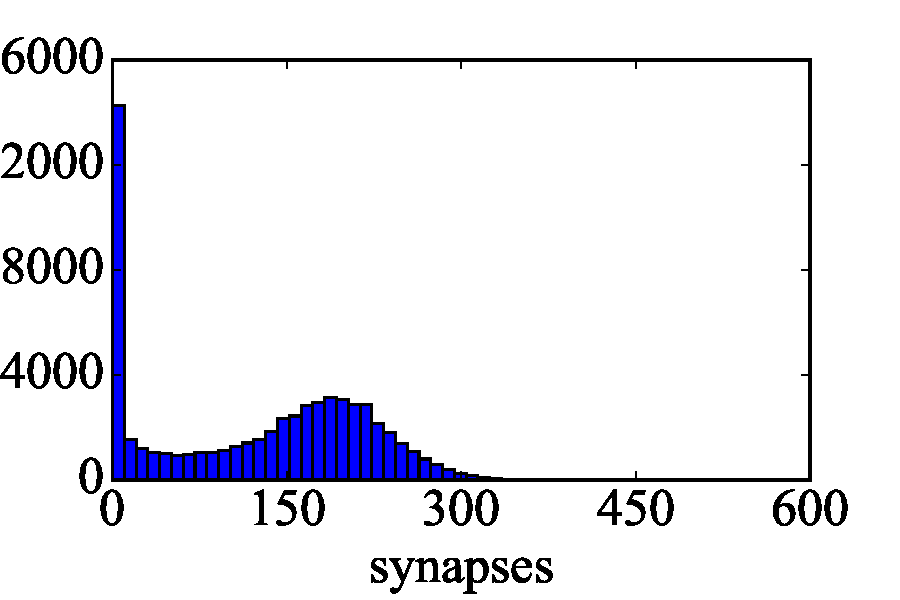
\includegraphics[scale=.3]{Fig5a}
  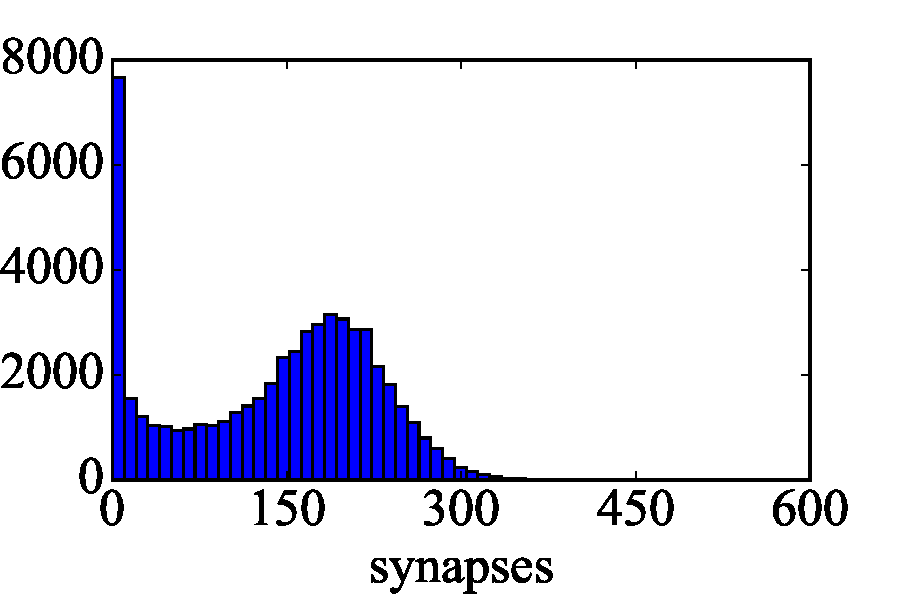
\includegraphics[scale=.3]{Fig5b}
  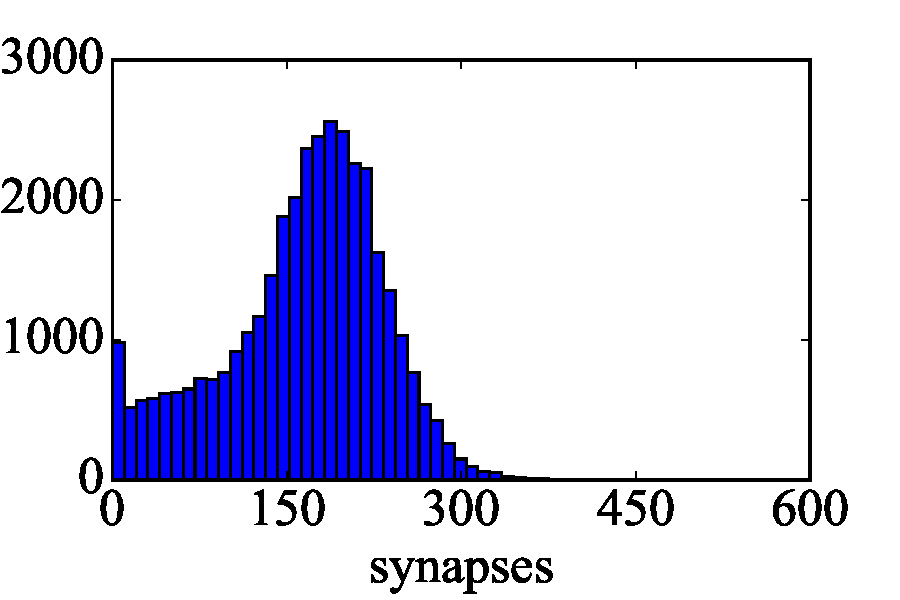
\includegraphics[scale=.3]{Fig5c}
  \caption{Left: raw data. Middle: remove unmasked = 0. Right: remove edges}
\end{figure} 

\subsection{Descriptive analysis}

With the data cleaned and cut into a relatively error-free data set, initial analysis can begin. This incorporates a broad look at the quality of the data in order to catch overarching features and ascertain basic characteristics.

\subsubsection{Image data verification}

The images that the data is based off of was also subject to scrutiny. Additional manual verification was done to determine possibility of a skew or bias in the image processing algorithms to determine synapse counts.

To begin with, a relationship between the data set and the analysis platform on \url{http://viz.neurodata.io/bock11/} was made. Based off of the x, y, and z ranges, it was determined that the data points matched with a magnification value of 5. Additionally, the z value was offset by 2917. Utilizing this information, one can find a rough estimate of a specific voxel indicated in the data set in the image.

Counting was done on the source images by hand, in order to confirm validity and accuracy of the synapse counting algorithm. The manual counting has inaccuracies as well, but it is unbiased and thus the errors will cancel each other out. The manual counts were performed at similar values of x, y, and z and then averaged. These data points were then collected across x, y, and z.

\begin{figure}[h]
  \centering
  \fbox{\rule[-.5cm]{0cm}{4cm} \rule[-.5cm]{4cm}{0cm}}
  \fbox{\rule[-.5cm]{0cm}{4cm} \rule[-.5cm]{4cm}{0cm}}
  \fbox{\rule[-.5cm]{0cm}{4cm} \rule[-.5cm]{4cm}{0cm}}
  \caption{Manual counts - data. Left: across x. Center: across y. Right: across z.}
\end{figure}

The fact that the data exhibits XXX indicates XXX.

\subsubsection{Describing unmasked}

Earlier it was explained that a relationship exists between the unmasked value and how much of the voxel is readable. Investigating further, it makes sense that unmasked values would correspong to synapse density values. We see that this is true, with a correlation of 0.896.

Since each voxel may have a different value for unmasked, which correlates to its synaptic density, it is important for us to account for this difference. The normalization is quite straightforward - \[normalized = synapse/unmaked \]

This new normalized value accounts for unmasked values in the synapse density data, and is a better choice for data analysis in this situation.

If one only used synapse values, the possibility of a bias due to localized unmasked values would prevents the results from remaining sound in the face of further testing.

\subsubsection{Preliminary trends}

Using the normalized data, a brief glance at the data can generate initial features. Simply binning the data into slices in the xy-plane, xz-plane, and yz-plane can provide interesting insights. As one can see from the figures, there is a small change across x and z, while a visual decrease across y is apparent. If one looks more closely at the change in y, by examining the derivative of the plot, one finds an interesting pattern.

\begin{figure}[h]
  \centering
  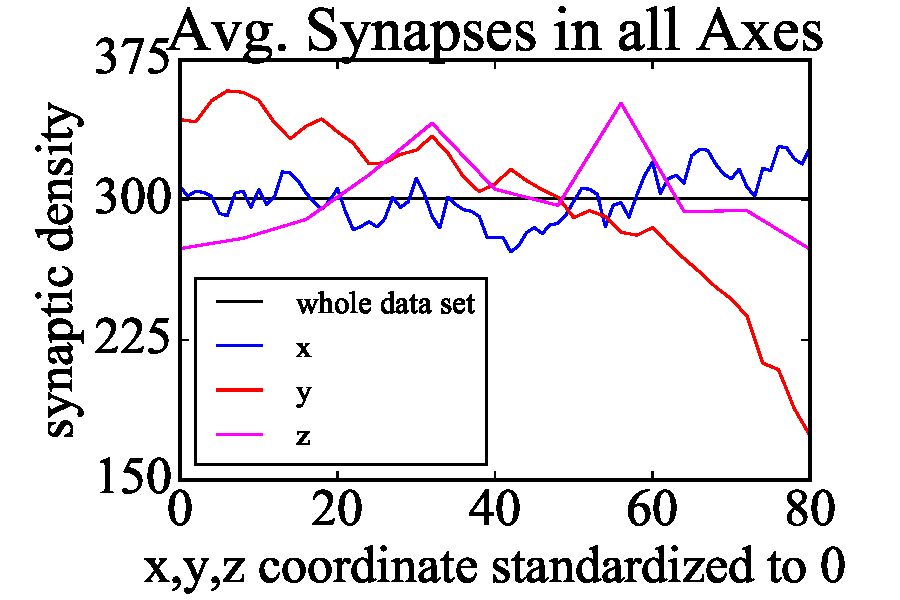
\includegraphics[scale=.3]{Fig7a}
  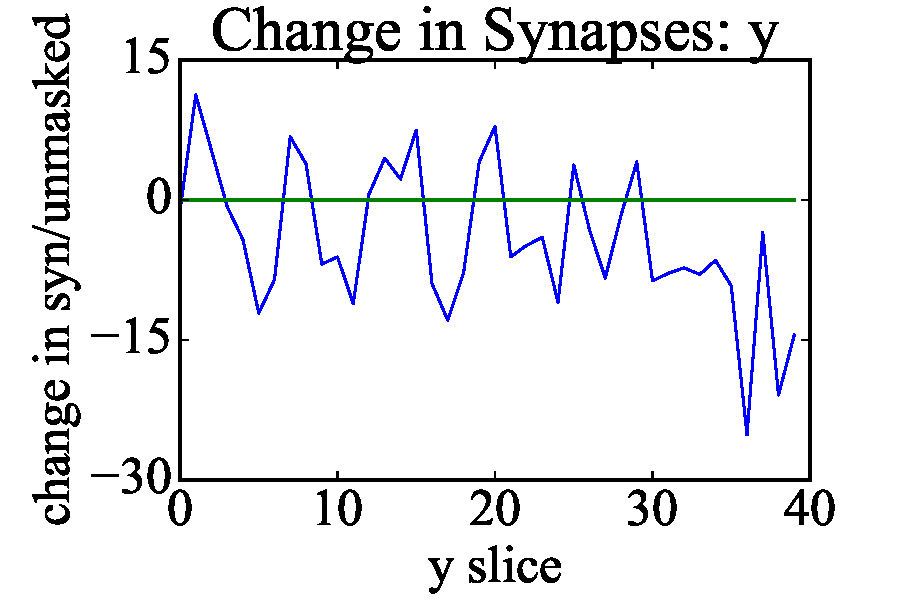
\includegraphics[scale=.3]{Fig7b}
  \caption{Left: Normalized values binned into planes. Right: derivative across y.}
\end{figure}

The wave-like pattern could either be attributed to noise, or an actual pattern in the data set. A smoothing function called b-spline was used to smooth the data, and can be seen below for both the change in y as well as its derivative.

\begin{figure}[h]
  \centering
  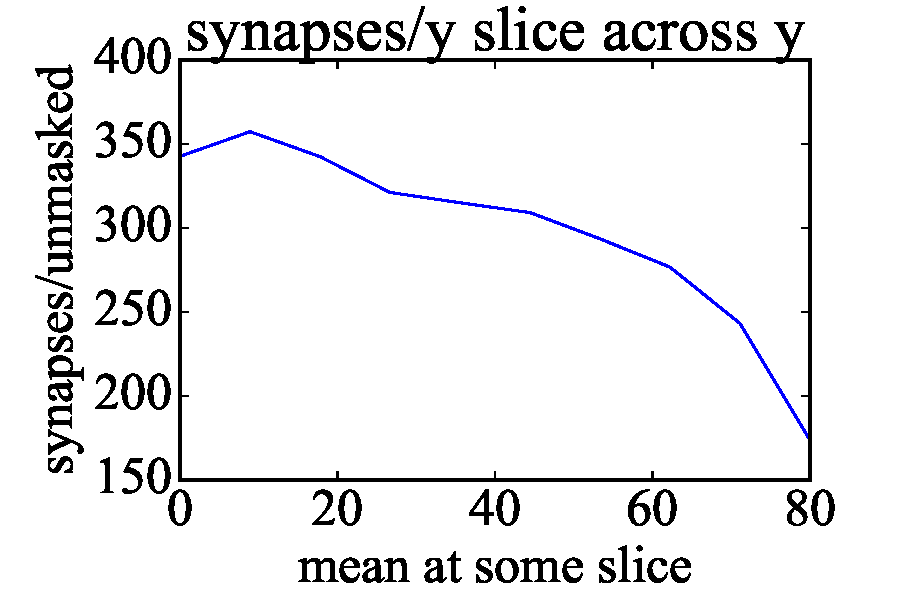
\includegraphics[scale=.3]{Fig8a}
  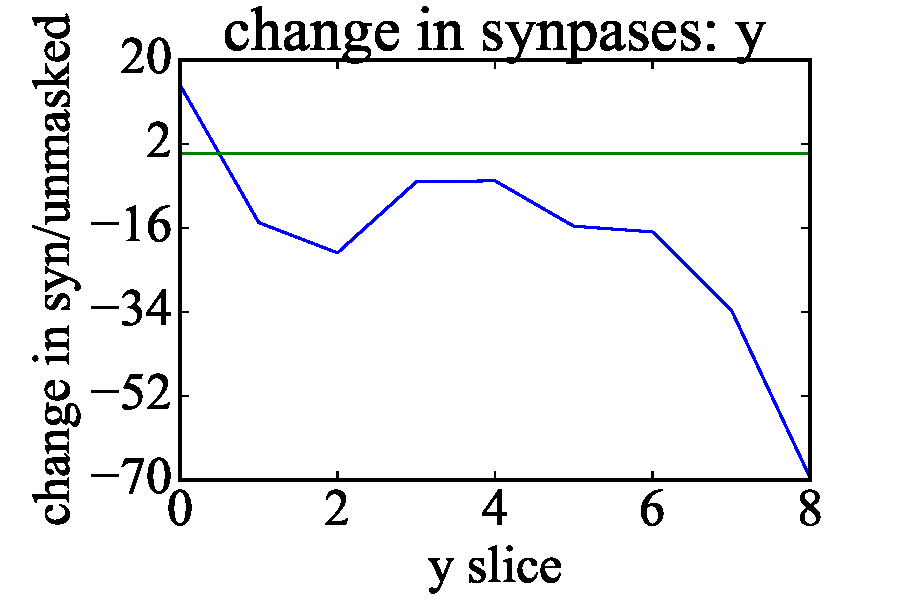
\includegraphics[scale=.3]{Fig8b}
  \caption{Left: smoothed normalized values across y. Right: smoothed derivative across y.}
\end{figure}

\subsection{Testing assumptions}

In order to correctly utilize some algorithms such as KNN, the assumptions about the data need to be tested. This will provide additional confidence in the results. 

\subsubsection{Synapse distribution uniformity}

A chi squared test can be used to determine uniformity - comparing the expected value of synapse density from the null hypothesis with the actual value at a certain bin. The equation is as follows - \[ X^2 = \Sigma((observed - expected)^2 /expected) \]
With specifically \[ H_o = Data\ uniformly\ distributed \] \[H_a =  Data\ not\ uniformly\ distributed \]

The expected density was generated simply by dividing the total number of synapses by the total number of data points.

The chi squared test returned a p-value of about 0. This implies that the data is not uniformly distributed and we reject the null hypothesis.

Furthermore, a justification of using the chi squared test is needed. This is shown by plotting power for both the null and alternate hypotheses, as shown.

\begin{figure}[h]
  \centering
  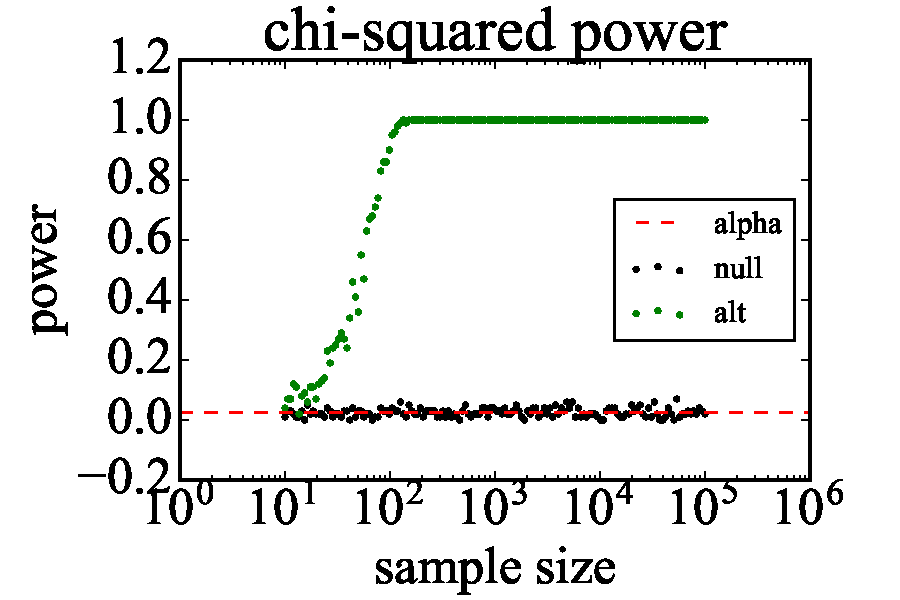
\includegraphics[scale = .3]{Fig9}
  \caption{Power under alternate hypothesis goes to 1, proving the claim.}
\end{figure}

\subsubsection{Identically and independently distributed (i.i.d.)}

Due to the nature of the data set, there is already a suspicion that the data is not i.i.d. Just looking at the image data  visually shows this.

The data was clustered using Gaussian mixture models (GMM) clustering, and a Bayesian Information Criteria (BIC) curve was generated. 

\begin{figure}[h]
  \centering
  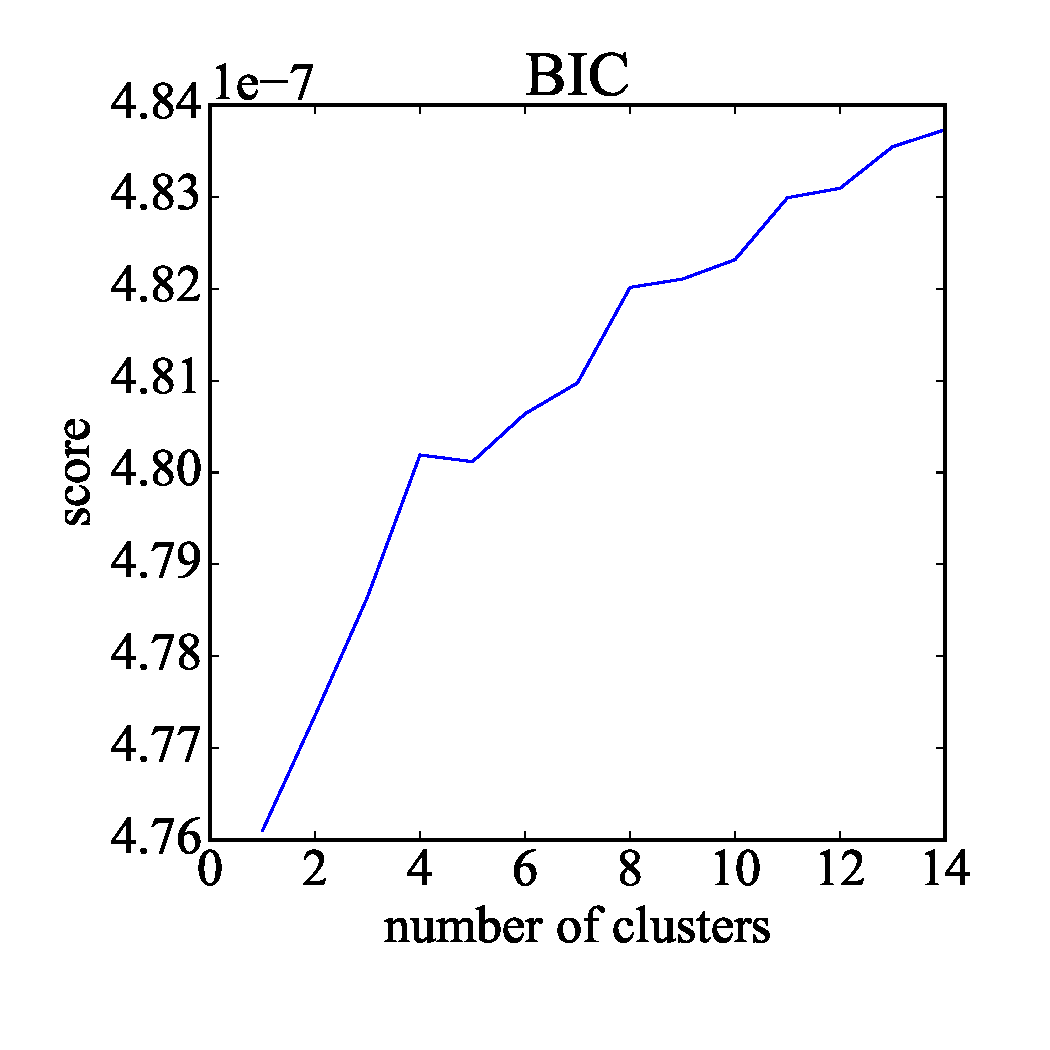
\includegraphics[scale = .3]{Fig10}
  \caption{An elbow can be seen at 4 clusters.}
\end{figure}

We additionally notice a jump at 11. The jump at 11 is most likely due to the fact that there are 11 z-values. This adds to the BIC since the z step is quite large, and any slight differences across z are magnified by this large step. The elbow at 4 indicates that the optimal number of clusters in this data set is 4. Since the optimal cluster is not one, the conclusion that the data is not identically distributed can be made.

To test independence, a covariance matrix between synapse density and spatial position can be generated. Due to the large data set, it is unfeasible to build a covariance matrix from the entire set. This can be replaced by an average of multiple covariance matrices generated from random sampling of the data set.

\begin{figure}[h]
  \centering
  \includegraphics[scale = .3]{Fig11}
  \caption{Covariance between synapse density and position.}
\end{figure}

As the covariance matrix is concentrated across the diagonal, the conclusion that the data is independently distributed can be made.

\subsection{Exploratory analysis}

\subsubsection{BIC curves for multiple z values}

Since a large spike in the overall BIC curve was found at 11 (11 unique z-values), perhaps each z value is distinct. Clustering across each z value removes the jump at 11 clusters.

\begin{figure}[h]
  \centering
  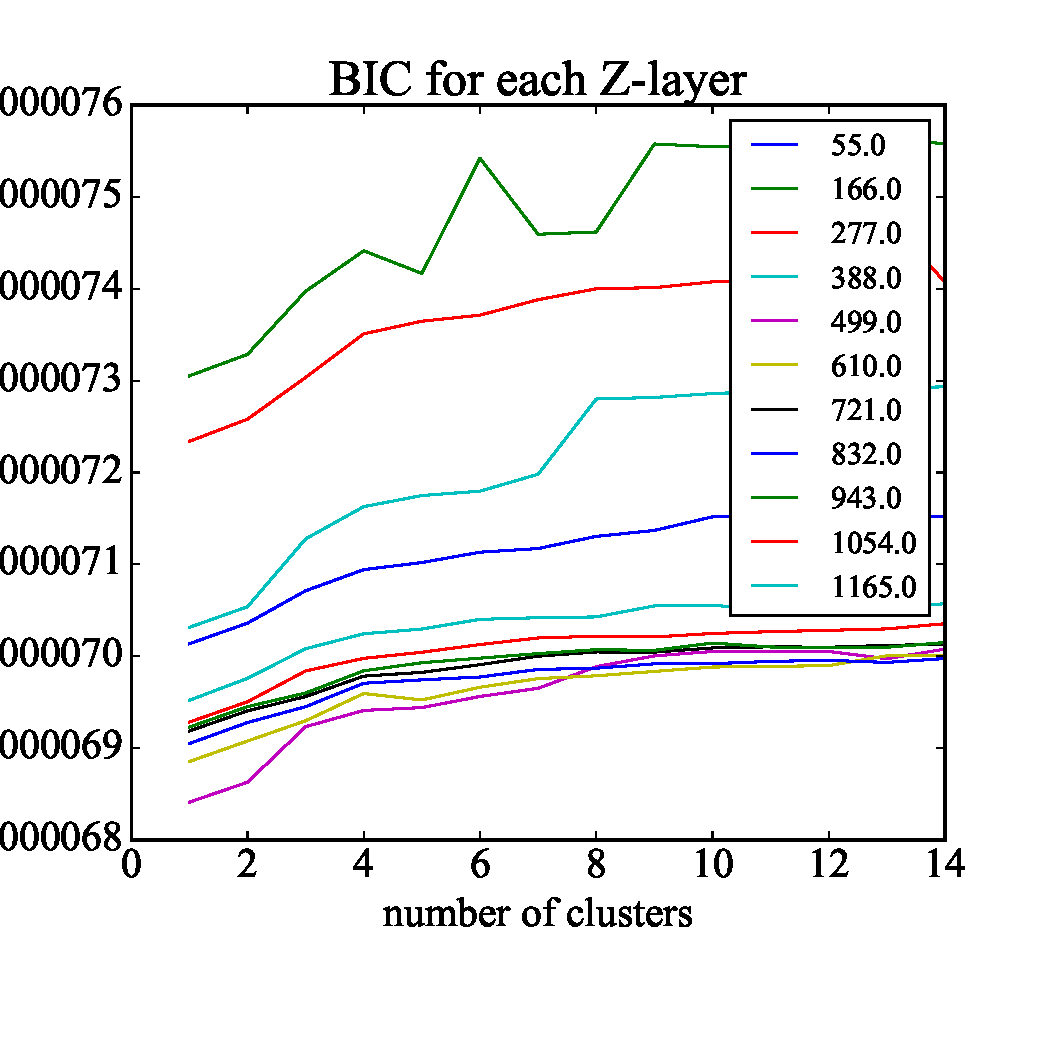
\includegraphics[scale=.3]{Fig12}
  \caption{BIC for each z-value.}
\end{figure}

\subsubsection{K-means clustering}

With all the assumptions tested, one can use K-means to cluster the data. The clustering was done for 4 clusters. The k-means clustering was also done on individual z-values.

\begin{figure}[h]
  \centering
  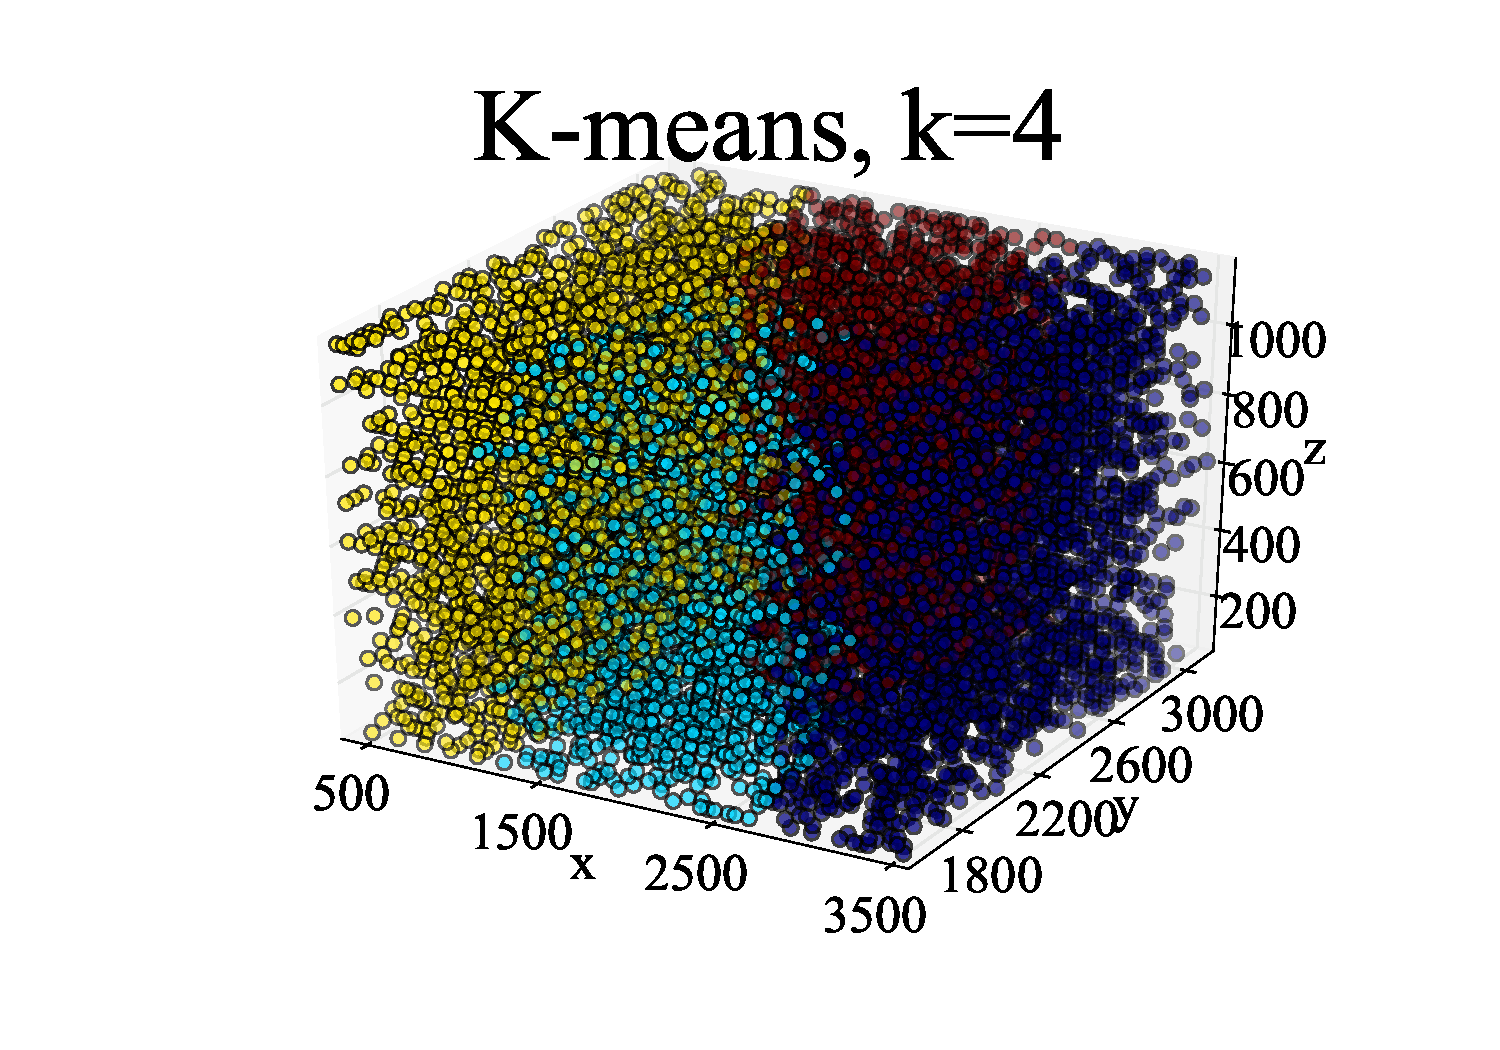
\includegraphics[scale=.15]{Fig13a}
  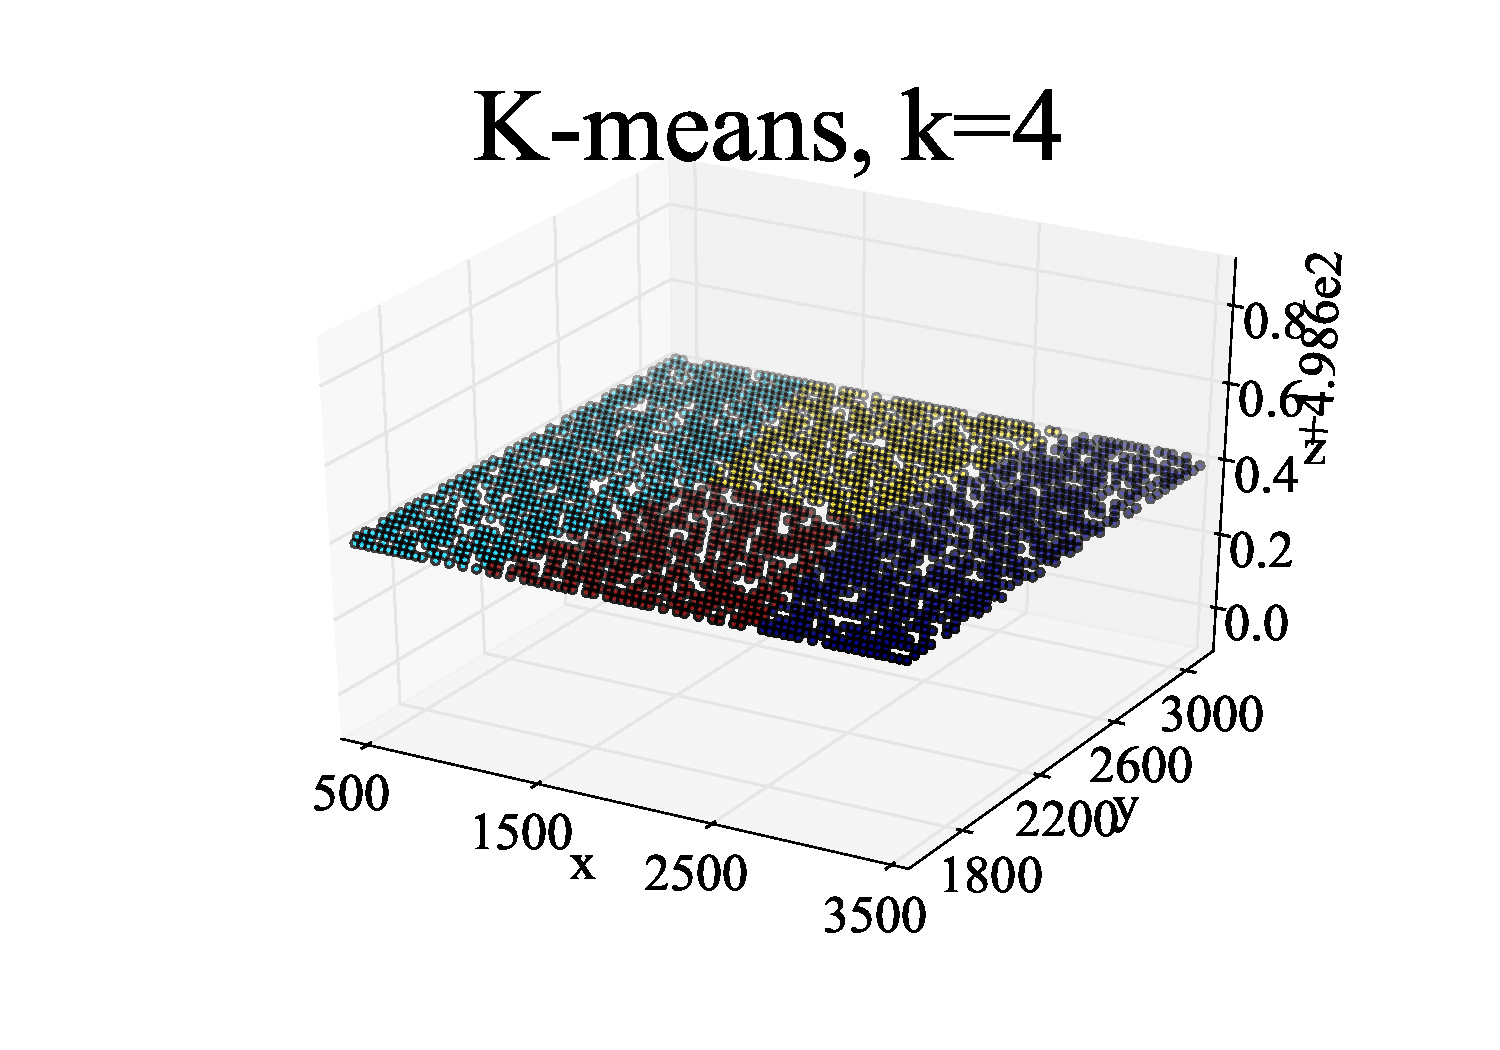
\includegraphics[scale=.15]{Fig13b}
  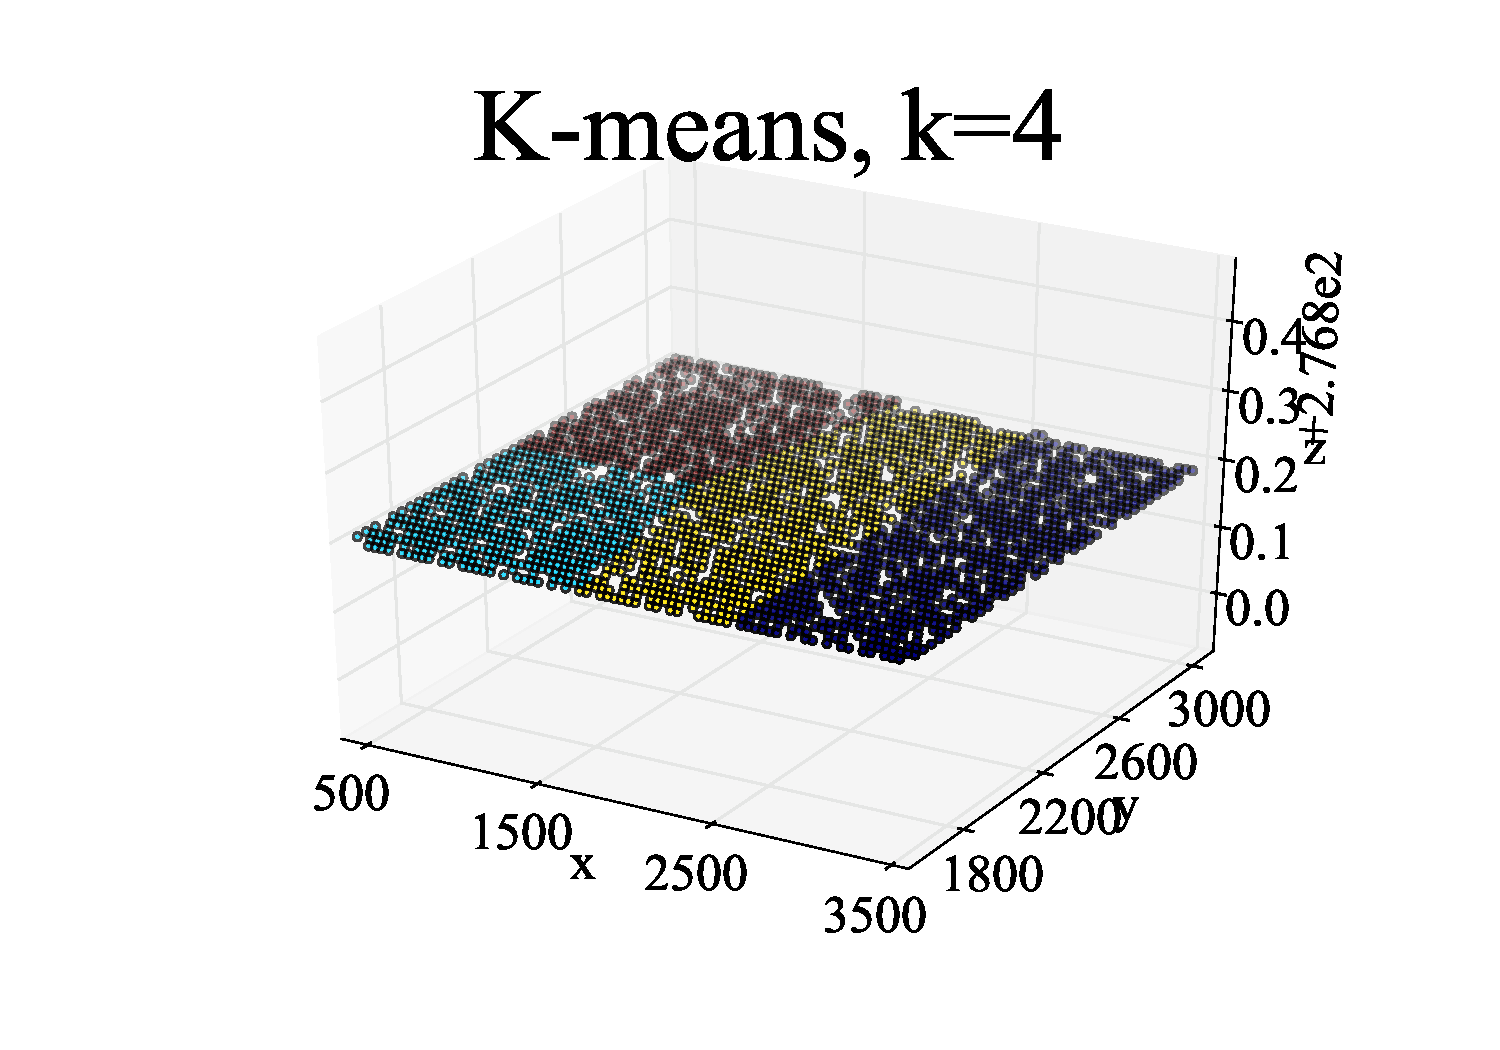
\includegraphics[scale=.15]{Fig13c}
  \caption{Left: Clustering in entire data set. Center: z = upper values. Right: z = lower values.}
\end{figure}

One can see that there is a definite change in synapse density across the y-axis. In terms of changes across z-values, it seems that whether the middle slice is split into two or the far slice is split into two depends on the z-value, as only the lower z values behave differently.

\section{Discussion}

The skew seen in the first figure of the results from the differences in manual vs computational acquisition of number of synapses does not truly change our conclusions, but simply further defines the nature of the data set. As seen from the results, a very strong trend of changes in synaptic density was observed across y. This follows the statements made by the paper that provided the data (Bock, et al. 2011). Yet, with deeper analysis, additional trends were observed. The changes in BIC curves when incorporating all z-values vs. a single one imply that there is a difference in synapse density between z-values. This was confirmed with K-means clustering, where clusters exhibited different behavior depending on their z-value. Whether part of this is a result of the skew in data is up to discussion

\section{Next steps}

The next task at hand is to try to identify this change in clustering across z-values. The interesting results using the k-means algorithm should be tested with other clustering algorithms. Additionally, the skew found is still only preliminary, and a more thorough manual counting should be done across more data points to increase the resolution of the skew. Schuz and Palm(1989) suggest that synapse density remains the same, and that neuron density is what changes. This suggests a re-evaluation of our counting algorithm. DeFelipe et al. (1999) suggests alternative estimaters, which we could compare to our own counts. Additionally, the Bock paper mentions the 2 main classes of synapses as being excitatory or inhibitory. Updating a data set to include these different classes of synapse could allow for a better model to be constructed.

\section{Future implications}

The implication of the results found are quite interesting. The potential that synaptic density can change within cortical layers would imply that, even within cortical layers, there are different zones of synaptic densities.

\section{References}

[1] Bock D, Lee W, Kerlin A, Andermann M, Hood G, Wetzel A, Yurgenson S, Soucy E, Kim H, Reid R. (2011). {\it Network anatomy and in vivo physiology of visual cortical neurons}. Nature article.

[2] Burette A, Collman F, Micheva K, Smith S and Weinberg R. (2015) {\it Knowing a synapse when you see one}. Frontiers in Neuroanatomy.

[3] Dani A, Huang B, Bergan J, Dulac C, Zhuang X. (2010). {\it Superresolution imaging of chemical synapses in the brain}. PubMed article.

[4] DeFelipe J, Marco P, Ignacio B, Merchan-Perez A. (1999) {\it Estimation of the Number of Synapses in the Cerebral Cortex: Methodological Considerations}. Cerebral Cortex.

[5] Koffie R, Hyman B, Spires-Jones T. (2011). {\it Alzheimer's disease: synapses gone cold}. BioMed Central article.

[6] Merchant P, Sulzer D, Sames D. (2015). {\it Synaptic optical imaging platforms: Examining pharmacological modulation of neurotransmitter release at discrete synapses}. ScienceDirect article.

[7] Scheff S, DeKosky S, Price D. (1990). {\it Quantitative assessment of cortical synaptic density in Alzheimer's disease}. ScienceDirect article.

[8] Schuz A, Palm G. (1989) {\it Density of neurons and synapses in the cerebral cortex of the mouse.}. PubMed article.

[9] Van Horn S, Ersir A, Sherman S. (2000). {\it Relative Distribution of Synapses in the
A-Laminae of the Lateral Geniculate
Nucleus of the Cat}. J of Comparatice Neurology article.

\section{Figures}

[1] Figure: \url{hoho.haha.shrapnel}, Code: \url{you got peeped!}

\end{document}